\chapter{Flow Control, Procedures, and Stack Management}

\section*{Learning Objectives}
After completing this experiment, you will be able to:
\begin{itemize}[nosep]
  \item Implement conditional and unconditional branching using ARM branch instructions.
  \item Design and implement loop constructs (\texttt{for}, \texttt{while}) using compare and branch instructions.
  \item Create and call procedures with proper parameter passing and return mechanisms.
  \item Manage the stack for local variables, parameter passing, and nested procedure calls.
  \item Apply the ARM Procedure Call Standard (AAPCS) to ensure correct register usage and calling conventions.
\end{itemize}

\section*{Experiment Overview}
This experiment introduces program control flow, procedure implementation, and stack management on the ARM Cortex-M4 processor. 
You will learn how to control program execution using branches and loops, create modular and reusable code using procedures, and manage memory efficiently through stack operations.

\noindent In this experiment, you will:
\begin{itemize}[nosep]
  \item Implement conditional branches and loop structures at the assembly level.
  \item Write and call procedures that follow standard calling conventions.
  \item Handle nested calls and parameter passing using the stack.
  \item Observe and analyze how the stack changes during procedure entry and return.
\end{itemize}

By the end of this lab, you will understand how to use branching and looping for program control, write well-structured procedures that follow AAPCS rules, and manage the stack during function calls and nested procedures.

\newpage
\etocsetnexttocdepth{subsubsection}
\localtableofcontents
\bigskip
\newpage
\section{Theoretical Background}
\subsection{Flow Control}
Flow control instructions alter the sequential execution of instructions by changing the program counter (PC). These instructions enable the implementation of conditional statements, loops, and procedure calls that are fundamental to structured programming.

\subsubsection{Condition Evaluation}
Before implementing control flow, we must understand how to evaluate conditions and set processor flags. ARM provides dedicated instructions for comparing values and testing bit patterns that update the condition flags without storing results.

\begin{table}[H]
\centering
\caption{ARM Cortex-M4 Compare and Test Instructions}
\small
\begin{tabularx}{\linewidth}{@{}l l X@{}}
\toprule
\textbf{Instr.} & \textbf{Syntax} & \textbf{Description / Usage} \\
\midrule
CMP     & \texttt{CMP Rn, Operand2}   & Compare \texttt{Rn} with \texttt{Operand2} (\texttt{Rn - Operand2}); updates flags (Z, N, C, V). \\
CMN     & \texttt{CMN Rn, Operand2}   & Compare negative (\texttt{Rn + Operand2}); used for checking against negative values. \\
TST     & \texttt{TST Rn, Operand2}   & Logical AND test (\texttt{Rn AND Operand2}); sets Z if all tested bits are 0. \\
TEQ     & \texttt{TEQ Rn, Operand2}   & Logical XOR test (\texttt{Rn EOR Operand2}); sets Z if operands are equal. \\
\bottomrule
\end{tabularx}
\end{table}

\paragraph{Usage Notes:}
\begin{itemize}[nosep]
  \item These instructions only affect the condition flags (N, Z, C, V) — they do not store a result.
  \item \texttt{CMP}/\texttt{CMN} are arithmetic comparisons; \texttt{TST}/\texttt{TEQ} are logical bitwise comparisons.
  \item Many data-processing instructions can update flags by appending \texttt{S} (e.g., \texttt{ADDS}, \texttt{SUBS}).
  \item Common use: immediately followed by conditional branches such as \texttt{BEQ}, \texttt{BNE}, \texttt{BGT}, etc.
\end{itemize}

\noindent\paragraph{Examples:}
\hfill
\begin{lstlisting}[caption={Arithmetic comparison using CMP}]
    CMP     R0, #10          ; Compare R0 with 10
    BLT     LessThan10       ; Branch if R0 < 10
    BGE     GreaterOrEqual   ; Otherwise, R0 >= 10
\end{lstlisting}

\begin{lstlisting}[caption={Bit test using TST}]
    MOV     R1, #0x12        ; R1 = 0001 0010b
    TST     R1, #0x10        ; Test if bit 4 is set
    BEQ     BitClear         ; Branch if bit 4 = 0 (Z=1)
    BNE     BitSet           ; Branch if bit 4 = 1 (Z=0)
\end{lstlisting}

\begin{lstlisting}[caption={Equality check using TEQ}]
    MOV     R2, #0x55
    MOV     R3, #0x55
    TEQ     R2, R3           ; XOR -> result 0, sets Z=1
    BEQ     ValuesEqual      ; Branch if equal
\end{lstlisting}

\subsubsection{Conditional Branching}
Branch instructions are the primary mechanism for implementing flow control in ARM assembly. They modify the program counter to jump to different parts of the code based on conditions or unconditionally.

\begin{table}[H]
\centering
\caption{ARM Cortex-M4 Branch Instructions}
\small
\begin{tabularx}{\linewidth}{@{}l l X@{}}
\toprule
\textbf{Instr.} & \textbf{Syntax} & \textbf{Description / Usage} \\
\midrule
B       & \texttt{B label}        & Unconditional branch to \texttt{label} (always jumps) \\
B\texttt{<cond>} & \texttt{B<cond> label}  & Conditional branch based on flags \\
BL      & \texttt{BL label}       & Branch with link: calls a subroutine, storing return address in \texttt{LR}. \\
BX      & \texttt{BX Rm}          & Branch to address in register, often \texttt{BX LR} to return from a subroutine. \\
CBZ     & \texttt{CBZ Rn, label}  & Branch if \texttt{Rn == 0}. Example: \texttt{CBZ R0, Done}. \\
CBNZ    & \texttt{CBNZ Rn, label} & Branch if \texttt{Rn != 0}. Example: loop until counter reaches zero. \\
\bottomrule
\end{tabularx}
\end{table}

\paragraph{\texttt{CBZ/CBNZ}} instructions have specific constraints:
\begin{itemize}[nosep]
  \item \textbf{Register}: operand must be a low register \texttt{R0--R7}.
  \item \textbf{Range}: branch is \emph{forward-only}; the destination must be within 0--126 bytes after the instruction.
  \item \textbf{Flags}: does not update condition flags (\texttt{N, Z, C, V}).
\end{itemize}
For backward or longer jumps, use \texttt{CMP}/\texttt{TST} with conditional branches (\texttt{BEQ}, \texttt{BNE}, \texttt{BGT}, \dots).

\subsubsection{Conditional Execution}
ARM assembly supports conditional execution, where most instructions can be conditionally executed based on the current state of the condition flags. This feature allows for efficient implementation of conditional statements without explicit branching.

\paragraph{Conditional Instruction Format:}
Most ARM instructions can be made conditional by appending a condition code suffix:
\[
\texttt{OPCODE\{<cond>\} Rd, Rn, Operand2}
\]

\paragraph{Examples:}
\begin{itemize}[nosep]
    \item \texttt{ADDEQ R0, R1, R2} — Add only if equal (Z=1)
    \item \texttt{MOVNE R3, \#10} — Move only if not equal (Z=0)
    \item \texttt{SUBGT R4, R4, \#1} — Subtract only if greater than (signed)
\end{itemize}

\paragraph{Advantages of Conditional Execution:}
\begin{itemize}[nosep]
    \item \textbf{Performance}: Eliminates branch instructions for simple conditional operations
    \item \textbf{Code density}: Reduces the number of instructions needed
    \item \textbf{Pipeline efficiency}: Avoids branch prediction penalties for simple conditions
    \item \textbf{Atomic operations}: Multiple related conditional operations can be grouped
\end{itemize}
\subsubsection{How Branch Instructions Work}

Branch instructions change the flow of execution by modifying the Program Counter (\texttt{PC}). 
When a branch is executed, the instruction encodes an \emph{offset} which is added to the current value of the \texttt{PC}.

\paragraph{Offset calculation:}  
The branch instruction contains a signed immediate value (positive or negative).  
The processor adds this offset (aligned to halfword boundaries) to the current \texttt{PC}.  
\begin{itemize}
    \item A \emph{positive offset} causes a \textbf{forward branch} (jump to a higher memory address, later in the program).  
    \item A \emph{negative offset} causes a \textbf{backward branch} (jump to a lower memory address, earlier in the program).  
\end{itemize} 

\paragraph{Example:}  
Suppose a branch instruction is located at address \texttt{0x100}, and the assembler encodes an immediate offset of \texttt{-0x08}.  
The effective target address will be:
\[
0x100 + 4 + (-0x08) = 0xFC
\]
This means the processor jumps \textbf{backward} to an earlier instruction.  
Such negative offsets are typically used to implement loops (e.g., repeat until zero).

\subsubsection{Condition Codes}
Conditional branches use condition codes that test the processor status flags (N, Z, C, V) set by previous instructions. These enable implementing high-level constructs like if-statements and loops.

\begin{table}[H]
\centering
\caption{Common ARM Condition Codes}
\small
\begin{tabularx}{0.72\linewidth}{@{}l l X@{}}
\toprule
\textbf{Cond.} & \textbf{Meaning} & \textbf{Description} \\
\midrule
EQ  & Equal                     & Execute if $Z=1$. \\
NE  & Not equal                 & Execute if $Z=0$. \\
CS/HS & Carry set / Unsigned higher or same & Execute if $C=1$. \\
CC/LO & Carry clear / Unsigned lower        & Execute if $C=0$. \\
MI  & Minus (negative)          & Execute if $N=1$. \\
PL  & Plus (non-negative)       & Execute if $N=0$. \\
VS  & Overflow set              & Execute if $V=1$. \\
VC  & Overflow clear            & Execute if $V=0$. \\
HI  & Unsigned higher           & Execute if $C=1$ \emph{and} $Z=0$. \\
LS  & Unsigned lower or same    & Execute if $C=0$ \emph{or} $Z=1$. \\
GE  & Greater or equal (signed) & Execute if $N=V$. \\
LT  & Less than (signed)        & Execute if $N\neq V$. \\
GT  & Greater than (signed)     & Execute if $Z=0$ \emph{and} $N=V$. \\
LE  & Less or equal (signed)    & Execute if $Z=1$ \emph{or} $N\neq V$. \\
AL  & Always                    & Always execute (default if no condition). \\
NV  & Never                     & Reserved / do not use. \\
\bottomrule
\end{tabularx}
\end{table}

\subsection{Loop Patterns}
Loops are fundamental control structures that repeat a block of code based on conditions. ARM assembly implements loops using combinations of compare instructions, conditional branches, and counters.

\subsubsection{For Loop Structure}
A typical for loop has the structure: initialization, condition check, body execution, and increment/decrement. This type of loop executes a known number of times.
\begin{lstlisting}[caption={Declaring Array and Length}]
        AREA M_DATA, DATA, READONLY
array   DCD 10, 20, 30, 40, 50   ; array of 5 integers
length  EQU 5                    ; number of elements (; just a constant, no memory)
\end{lstlisting}
\begin{lstlisting}[caption={For loop implementation pattern}]
        ; Initialization
        MOV     R0, #0                  ; i = 0
        MOV     R1, #0                  ; sum = 0
        LDR     R3, =array              ; load base address of array into R3

for_start
        ; Condition check
        CMP     R0, #length             ; compare i with length
        BGE     for_end                 ; if i >= length, exit loop

        ; Loop body
        LDR     R2, [R3, R0, LSL #2]    ; load array[i]; EA: R3 + (R0 * 4)
        ADD     R1, R1, R2              ; sum += array[i]

        ; Increment
        ADD     R0, R0, #1              ; i++
        B       for_start               ; repeat

for_end
\end{lstlisting}
\subsubsection{While Loop Structure}
While loops check the condition before executing the loop body, potentially executing zero times if the initial condition is false. This type of loop is useful when the number of iterations is not known in advance and depends on dynamic conditions.
\begin{lstlisting}[caption={Declaring Null-Terminated String}]
        AREA M_DATA, DATA, READONLY
mystring DCB "Hello World!", 0    ; null-terminated string
\end{lstlisting}
\paragraph{Note:} \texttt{0} and \texttt{'0'} are two different values, as the former is actually zero, while the latter is the ASCII code for the character '0' (which is 48 in decimal).
\newpage

\begin{lstlisting}[caption={While loop with string processing example}]
    ; Intialization
    LDR     R0, =mystring   ; pointer to string
    MOV     R1, #0          ; character count = 0

while_start
                            ; Condition check
    LDRB    R2, [R0], #1    ; load current character and post-increment pointer
    CMP     R2, #0          ; check for null terminator
    BEQ     while_end       ; if zero, exit loop
    
                            ; Loop body - do something with R2

    
    B       while_start     ; repeat
while_end
\end{lstlisting}


\subsection{Procedures and Stack}

\subsubsection{ARM Architecture Procedure Call Standard (AAPCS)}

Procedures are reusable blocks of code that encapsulate a specific task. They promote modular design, code reuse, and clearer program structure. In ARM assembly, procedures are implemented using branch-and-link instructions along with register usage conventions defined by the ARM Architecture Procedure Call Standard (AAPCS).

The AAPCS is the set of rules that define how functions exchange data and how registers must be preserved during a procedure call:

\begin{itemize}[nosep]
  \item \textbf{R0--R3}: Hold the first four parameters. \texttt{R0} also holds the return value. Caller-saved.
  \item \textbf{Stack}: Any additional parameters beyond the first four are passed on the stack.
  \item \textbf{R4--R11}: Must be preserved by the callee. If a procedure uses them, it must save and restore them. 
  \item \textbf{SP (R13)}: Stack pointer, always points to the current top of the stack.
  \item \textbf{LR (R14)}: Link register holds the return address. Caller-saved.
\end{itemize}
\paragraph{Note:} Callees are the procedures being called, while callers are the ones calling the procedure.

\subsubsection{Procedure Templates}

A procedure is entered with a \texttt{BL} (branch-with-link) instruction, which stores the return address in the link register \texttt{LR}. The callee returns by branching to \texttt{LR} (e.g., \texttt{BX LR}). By the AAPCS, the first four arguments are passed in \texttt{R0--R3} and the primary return value is placed in \texttt{R0}.
\newpage
\paragraph{Basic Procedure Template}

\paragraph{Example:} simple procedure that expects two integers in \texttt{R0} and \texttt{R1} and returns their sum in \texttt{R0}.

\begin{lstlisting}[caption={Basic procedure structure}]
AddTwo  PROC
        ADD R0, R0, R1   ; return R0+R1 in R0
        BX  LR
        ENDP
\end{lstlisting}
\paragraph{Note:} The \texttt{PROC} and \texttt{ENDP} directives help define the start and end of a procedure and they could be safely omitted.

\paragraph{Procedure with Preserved Registers}

When a procedure uses callee-saved registers (R4-R11), it must preserve their original values by saving them on the stack and restoring them before returning:

\begin{lstlisting}[caption={Procedure using preserved registers}]
ProcessArray PROC
        PUSH    {R4-R6, LR}     ; Save used registers and LR
        MOV     R4, R0          ; Save array pointer
        MOV     R5, R1          ; Save array length  
        MOV     R6, #0          ; Initialize counter
        
        ; Process array using R4, R5, R6...
        
        MOV     R0, R6          ; Return counter value
        POP     {R4-R6, PC}     ; Restore registers and return
        ENDP
\end{lstlisting}

\paragraph{Nested Procedure Calls}

When one procedure calls another, the link register (\texttt{LR}) must be preserved, otherwise the return address would be lost. This is done by pushing \texttt{LR} onto the stack before making another call.

\begin{lstlisting}[caption={Nested procedure example}]
OuterProc
        PUSH    {LR}            ; Save return address
        BL      InnerProc       ; Call inner procedure
        MOV     R1, R0          ; Use return value
        POP     {PC}            ; Return to caller

InnerProc 
        MOV     R0, #42         ; Return value
        BX      LR              ; Return
\end{lstlisting}


\subsubsection{Stack Model (Full, Descending)}
There are four common stack models based on two characteristics: whether the stack is full or empty, and whether it grows up (ascending) or down (descending). 
\begin{itemize}[nosep]
    \item \textbf{Full Ascending}: SP points to the last used location; stack grows toward higher addresses.
    \item \textbf{Empty Ascending}: SP points to the next free location; stack grows toward higher addresses.
    \item \textbf{Empty Descending}: SP points to the next free location; stack grows toward lower addresses.
    \item \textbf{Full Descending}: SP points to the last used location; stack grows toward lower addresses.
\end{itemize}
The ARM Cortex-M4 uses a \textbf{full descending stack}, meaning:
\begin{itemize}[nosep]
    \item The stack pointer (\texttt{SP}) points to the last used location (full).
    \item The stack grows toward lower memory addresses (descending).
\end{itemize}
\subsubsection{Stack Operations}

The Cortex-M4 provides \texttt{PUSH} and \texttt{POP} instructions that automatically update the stack pointer (\texttt{SP}) and allow saving or restoring multiple registers in a single instruction.  
These operations are essential for implementing procedure calls, local variables, and context switching.
\paragraph{PUSH}

The \texttt{PUSH} instruction saves one or more registers onto the stack in a single operation.
When executed, the stack pointer (\texttt{SP}) is decremented to reserve space, and the specified registers are written to consecutive memory locations starting from the new \texttt{SP} value.
\textbf{Rule:} \texttt{PUSH} stores registers on the stack, with the \textbf{lowest-numbered register} placed at the \textbf{lowest memory address} and the \textbf{highest-numbered register} placed at the \textbf{highest memory address}.
This guarantees a consistent and predictable memory layout for saved contexts.

\medskip
\noindent
\textbf{Example:}
\begin{lstlisting}
    PUSH {R4, R0, R2, LR}
\end{lstlisting}

Even if the list appears unordered, values are laid out by register number: R0 (lowest address), then R2, R4, and LR (highest address).
Each register occupies 4 bytes, so \texttt{SP} decreases by 16 bytes in total.
The program counter (\texttt{PC}) cannot be pushed by this instruction.

\begin{figure}[H]
\centering
\begin{subfigure}[t]{0.3\textwidth}
    \centering
    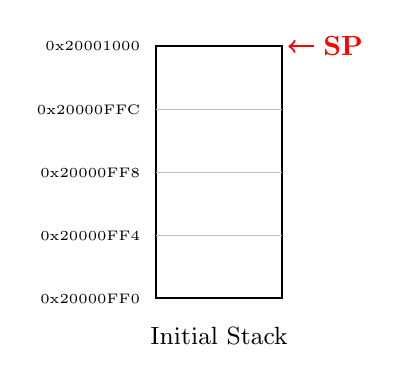
\begin{tikzpicture}[scale=0.8]
        % Stack frame
        \draw[thick] (0,0) rectangle (2,4);
        
        % Grid lines for 4 cells
        \foreach \y in {1,2,3} {
            \draw[thin, gray!50] (0,\y) -- (2,\y);
        }
        
        % Memory addresses (descending)
        \node[anchor=east] at (-0.1,4) {\tiny 0x20001000};
        \node[anchor=east] at (-0.1,3) {\tiny 0x20000FFC};
        \node[anchor=east] at (-0.1,2) {\tiny 0x20000FF8};
        \node[anchor=east] at (-0.1,1) {\tiny 0x20000FF4};
        \node[anchor=east] at (-0.1,0) {\tiny 0x20000FF0};
        
        % Stack pointer arrow
        \draw[->, thick, red] (2.5,4) -- (2.1,4);
        \node[right, red] at (2.5,4) {\textbf{SP}};
        
        % Title
        \node[below] at (1,-0.3) {\small Initial Stack};
    \end{tikzpicture}
    \caption{Initial empty stack}
    \label{fig:stack-initial}
\end{subfigure}
\hfill
\begin{subfigure}[t]{0.3\textwidth}
    \centering
    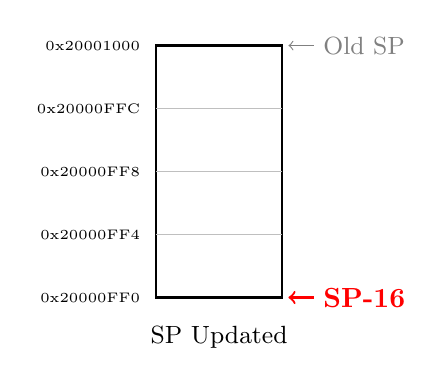
\begin{tikzpicture}[scale=0.8]
        % Stack frame
        \draw[thick] (0,0) rectangle (2,4);
        
        % Grid lines for 4 cells
        \foreach \y in {1,2,3} {
            \draw[thin, gray!50] (0,\y) -- (2,\y);
        }
        
        % Memory addresses (descending)
        \node[anchor=east] at (-0.1,4) {\tiny 0x20001000};
        \node[anchor=east] at (-0.1,3) {\tiny 0x20000FFC};
        \node[anchor=east] at (-0.1,2) {\tiny 0x20000FF8};
        \node[anchor=east] at (-0.1,1) {\tiny 0x20000FF4};
        \node[anchor=east] at (-0.1,0) {\tiny 0x20000FF0};
        
        % Old SP position (grayed out)
        \draw[->, thin, gray] (2.5,4) -- (2.1,4);
        \node[right, gray] at (2.5,4) {\small Old SP};
        
        % New SP position after PUSH {R0, R2, R4, LR}
        \draw[->, thick, red] (2.5,0) -- (2.1,0);
        \node[right, red] at (2.5,0) {\textbf{SP-16}};
        
        
        
        % Title
        \node[below] at (1,-0.3) {\small SP Updated};
    \end{tikzpicture}
    \caption{Stack pointer decremented}
    \label{fig:stack-sp-update}
\end{subfigure}
\hfill
\begin{subfigure}[t]{0.3\textwidth}
    \centering
    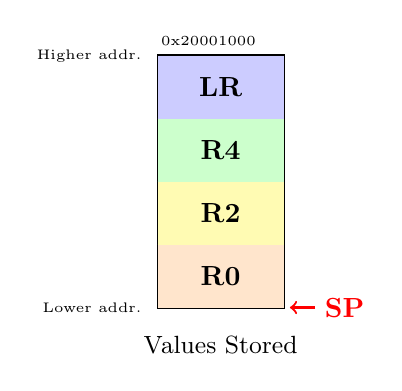
\begin{tikzpicture}[scale=0.8]
        % Stack frame
        \draw[thick] (0,0) rectangle (2,4);
        
        % Grid lines for 4 cells
        \foreach \y in {1,2,3} {
            \draw[thin, gray!50] (0,\y) -- (2,\y);
        }
        
        % Memory addresses (descending)
        \node[left, anchor=south west] at (-0.1,4) {\tiny 0x20001000};
        \node[left, anchor=south west] at (-0.1,3) {\tiny 0x20000FFC};
        \node[left, anchor=south west] at (-0.1,2) {\tiny 0x20000FF8};
        \node[left, anchor=south west] at (-0.1,1) {\tiny 0x20000FF4};
        \node[left, anchor=south west] at (-0.1,0) {\tiny 0x20000FF0};
        
        % Stored registers (in ascending order by number)
        \fill[blue!20] (0,3) rectangle (2,4);
        \node at (1,3.5) {\textbf{LR}};
        
        \fill[green!20] (0,2) rectangle (2,3);
        \node at (1,2.5) {\textbf{R4}};
        
        \fill[yellow!30] (0,1) rectangle (2,2);
        \node at (1,1.5) {\textbf{R2}};
        
        \fill[orange!20] (0,0) rectangle (2,1);
        \node at (1,0.5) {\textbf{R0}};
        
        % Stack pointer pointing to last used location
        \draw[->, thick, red] (2.5,0) -- (2.1,0);
        \node[right, red] at (2.5,0) {\textbf{SP}};
        
        % Annotations
        \node[left] at (-0.1,4) {\tiny Higher addr.};
        \node[left] at (-0.1,0) {\tiny Lower addr.};
        
        % Title
        \node[below] at (1,-0.3) {\small Values Stored};
    \end{tikzpicture}
    \caption{Registers stored in order}
    \label{fig:stack-values}
\end{subfigure}
\caption{Stack operation sequence for \texttt{PUSH \{R4, R0, R2, LR\}}}
\label{fig:stack-push-sequence}
\end{figure}

\noindent\textbf{Explanation:}
Figure~\ref{fig:stack-push-sequence}\textbf{(a)} shows the empty stack with \texttt{SP} at the top (highest address).
When \texttt{PUSH} executes, the processor \textbf{decrements \texttt{SP} by 16 bytes} to reserve space for four registers (Figure~\ref{fig:stack-push-sequence}\textbf{(b)}).
Finally, in Figure~\ref{fig:stack-push-sequence}\textbf{(c)}, values are stored according to the rule: the lowest-numbered register (R0) at the lowest address, then R2 and R4, and the highest-numbered (LR) at the highest address.
Because the stack grows downward, \texttt{SP} points to the last written word after the operation.

\bigskip
\paragraph{POP}

The \texttt{POP} instruction restores one or more registers from the stack.
Conceptually, the processor reads each value from the addresses currently covered by \texttt{SP} and then releases that stack space.
\textbf{Rule:} \texttt{POP} loads registers from the stack such that the \textbf{lowest-numbered register} is restored from the \textbf{lowest memory address}, and the \textbf{highest-numbered register} from the \textbf{highest memory address}.
After all specified registers are restored, \texttt{SP} has increased by 4 bytes per register.

\medskip
\noindent
\textbf{Example:}
\begin{lstlisting}
    POP {R6-R8}
\end{lstlisting}

This restores R6, then R7, then R8 from successively higher addresses; the stack pointer increases by 12 bytes overall.
If \texttt{PC} is included in the list, the loaded value becomes the new program counter, returning from the current procedure.

\begin{figure}[H]
\centering

\begin{subfigure}[t]{0.3\textwidth}
    \centering
    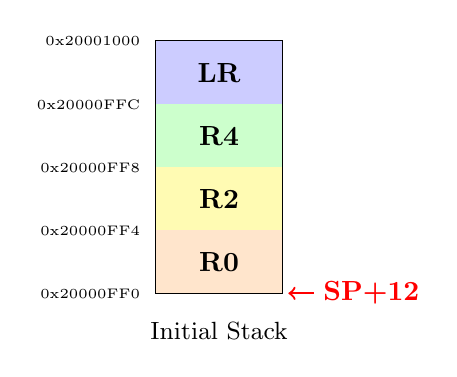
\begin{tikzpicture}[scale=0.8]
        % Stack frame
        \draw[thick] (0,0) rectangle (2,4);
        
        % Grid lines for 4 cells
        \foreach \y in {1,2,3} {
            \draw[thin, gray!50] (0,\y) -- (2,\y);
        }
        

        
        % Stored registers (in ascending order by number)
        \fill[blue!20] (0,3) rectangle (2,4);
        \node at (1,3.5) {\textbf{LR}};
        
        \fill[green!20] (0,2) rectangle (2,3);
        \node at (1,2.5) {\textbf{R4}};
        
        \fill[yellow!30] (0,1) rectangle (2,2);
        \node at (1,1.5) {\textbf{R2}};
        
        \fill[orange!20] (0,0) rectangle (2,1);
        \node at (1,0.5) {\textbf{R0}};
        
        % Stack pointer pointing to last used location
        \draw[->, thick, red] (2.5,0) -- (2.1,0);
        \node[right, red] at (2.5,0) {\textbf{SP+12}};
        
        % Annotations
        % Memory addresses (descending)
        \node[anchor=east] at (-0.1,4) {\tiny 0x20001000};
        \node[anchor=east] at (-0.1,3) {\tiny 0x20000FFC};
        \node[anchor=east] at (-0.1,2) {\tiny 0x20000FF8};
        \node[anchor=east] at (-0.1,1) {\tiny 0x20000FF4};
        \node[anchor=east] at (-0.1,0) {\tiny 0x20000FF0};
        
        % Title
        \node[below] at (1,-0.3) {\small Initial Stack};
    \end{tikzpicture}
    \caption{Initial stack after Figure \ref{fig:stack-push-sequence}}
\end{subfigure}
\hfill
\begin{subfigure}[t]{0.3\textwidth}
    \centering
    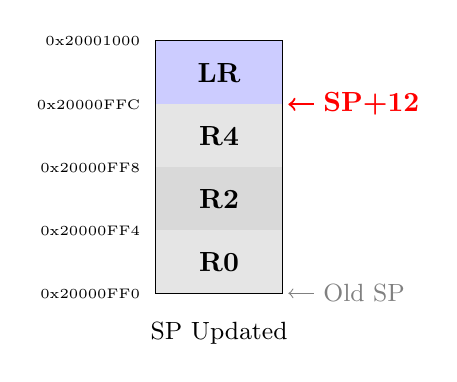
\begin{tikzpicture}[scale=0.8]
        % Stack frame
        \draw[thick] (0,0) rectangle (2,4);
        
        % Grid lines for 4 cells
        \foreach \y in {1,2,3} {
            \draw[thin, gray!50] (0,\y) -- (2,\y);
        }
        

        
        % Stored registers (in ascending order by number)
        \fill[blue!20] (0,3) rectangle (2,4);
        \node at (1,3.5) {\textbf{LR}};
        
        \fill[gray!20] (0,2) rectangle (2,3);
        \node at (1,2.5) {\textbf{R4}};
        
        \fill[gray!30] (0,1) rectangle (2,2);
        \node at (1,1.5) {\textbf{R2}};
        
        \fill[gray!20] (0,0) rectangle (2,1);
        \node at (1,0.5) {\textbf{R0}};
        
        % Stack pointer pointing to last used location
        \draw[->, thin, gray] (2.5,0) -- (2.1,0);
        \node[right, gray] at (2.5,0) {\small{Old SP}}; 

        \draw[->, thick, red] (2.5,3) -- (2.1,3);
        \node[right, red] at (2.5,3) {\textbf{SP+12}};
        
        % Annotations
        % Memory addresses (descending)
        \node[anchor=east] at (-0.1,4) {\tiny 0x20001000};
        \node[anchor=east] at (-0.1,3) {\tiny 0x20000FFC};
        \node[anchor=east] at (-0.1,2) {\tiny 0x20000FF8};
        \node[anchor=east] at (-0.1,1) {\tiny 0x20000FF4};
        \node[anchor=east] at (-0.1,0) {\tiny 0x20000FF0};
        
        % Title
        \node[below] at (1,-0.3) {\small SP Updated};
    \end{tikzpicture}
    \caption{Stack pointer incremented}
\end{subfigure}
\hfill
\begin{subfigure}[t]{0.3\textwidth}
    \centering
    \centering
    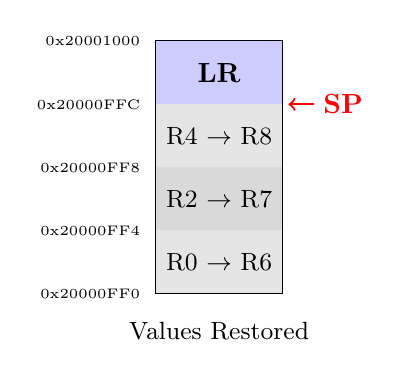
\begin{tikzpicture}[scale=0.8]
        % Stack frame
        \draw[thick] (0,0) rectangle (2,4);
        
        % Grid lines for 4 cells
        \foreach \y in {1,2,3} {
            \draw[thin, gray!50] (0,\y) -- (2,\y);
        }
        

        
        % Stored registers (in ascending order by number)
        \fill[blue!20] (0,3) rectangle (2,4);
        \node at (1,3.5) {\textbf{LR}};
        
        \fill[gray!20] (0,2) rectangle (2,3);
        \node at (1,2.5) {\small{R4 $\rightarrow$ R8}};
        
        \fill[gray!30] (0,1) rectangle (2,2);
        \node at (1,1.5) {\small{R2 $\rightarrow$ R7}};

        \fill[gray!20] (0,0) rectangle (2,1);
        \node at (1,0.5) {\small{R0 $\rightarrow$ R6}};
        
        % Stack pointer pointing to last used location
        \draw[->, thick, red] (2.5,3) -- (2.1,3);
        \node[right, red] at (2.5,3) {\textbf{SP}};
        
        % Annotations
        % Memory addresses (descending)
        \node[anchor=east] at (-0.1,4) {\tiny 0x20001000};
        \node[anchor=east] at (-0.1,3) {\tiny 0x20000FFC};
        \node[anchor=east] at (-0.1,2) {\tiny 0x20000FF8};
        \node[anchor=east] at (-0.1,1) {\tiny 0x20000FF4};
        \node[anchor=east] at (-0.1,0) {\tiny 0x20000FF0};
        
        % Title
        \node[below] at (1,-0.3) {\small Values Restored};
    \end{tikzpicture}
    \caption{Registers restored in order}
    \label{fig:stack-sp-update}
\end{subfigure}

\caption{Stack operation sequence for \texttt{POP \{R6-R8\}}}
\label{fig:stack-pop-sequence}
\end{figure}
\noindent\textbf{Explanation:}
In Figure~\ref{fig:stack-pop-sequence}\textbf{(a)}, the stack contains values saved earlier.
Executing \texttt{POP \{R6-R8\}} \textbf{reclaims 12 bytes of stack space} (three registers) by moving \texttt{SP} upward in memory (Figure~\ref{fig:stack-pop-sequence}\textbf{(b)}).
Then, as shown in Figure~\ref{fig:stack-pop-sequence}\textbf{(c)}, registers are restored following the rule: the lowest-numbered register (R6) comes from the lowest address, followed by R7 and R8 from higher addresses.
After the last load, \texttt{SP} points to the top of the reclaimed block, completing the reversal of the earlier push.



\newpage
\section{Procedure}

\subsection{Examples}

\subsubsection{Example 1: Array Example — Find Maximum Element}
This example demonstrates how to find the maximum element in an array using a standard for loop structure.
\lstinputlisting[caption={Find maximum element in an array}]{snippets/assembly/exp3/example1.asm}
\paragraph{Check:} Verify that the maximum element is correctly identified and stored in \texttt{MAXRES}.
\newpage

\subsubsection{Example 2: String Example — Count Uppercase Letters}
This example demonstrates how to process a null-terminated string and count the number of uppercase letters (A-Z) using a while-loop structure.
\lstinputlisting[caption={Count uppercase letters in a string}]{snippets/assembly/exp3/example2.asm}
\paragraph{Check:} Verify that the program correctly counts the uppercase letters and stores the result in \texttt{UPPERCOUNT}.

\newpage
\subsubsection{Example 3: Stack Example — Nested Uppercase Counter}
This example demonstrates a nested call: \texttt{CountUpperNested(ptr)} scans a null-terminated string and calls \texttt{IsUpper(ch)} for each character. It shows saving/restoring \texttt{LR} and using a callee-saved register (\texttt{R4}) for the running count.
\lstinputlisting[caption={Nested procedure call to count uppercase letters}]{snippets/assembly/exp3/example3.asm}
\paragraph{Check:} Verify that \texttt{UPPERCOUNT} contains \texttt{5} for the test string.

\newpage
\subsection{Tasks}

\subsubsection{Task 1: Count Vowels in a String}
Implement procedures to process strings with the following requirements:
\begin{itemize}[nosep]
    \item Create a procedure \texttt{CountVowels} that takes a string pointer in R0 and returns the number of vowels (a, e, i, o, u) in R0.
    \item Use nested procedure calls where \texttt{CountVowels} calls a helper procedure \texttt{IsVowel}.
    \item Follow AAPCS conventions for parameter passing and register usage.
\end{itemize}

\subsubsection{Task 2: Factorial Calculation (Iterative)}
Implement a procedure to calculate the factorial of a non-negative integer:
\begin{itemize}[nosep]
    \item Create a procedure \texttt{Factorial} that takes a non-negative integer in R0 and returns its factorial in R0.
    \item Use an iterative approach with a loop to compute the factorial.
    \item Ensure proper handling of edge cases, such as 0! = 1.
    \item Follow AAPCS conventions for parameter passing and register usage.
\end{itemize}
\subsubsection{Task 3: Factorial Calculation (Recursive)}
Implement a recursive version of the factorial calculation:
\begin{itemize}[nosep]
    \item Create a procedure \texttt{FactorialRec} that takes a non-negative integer in R0 and returns its factorial in R0.
    \item Use recursion to compute the factorial, ensuring proper base case handling.
    \item Manage the stack appropriately to save and restore registers as needed.
    \item Follow AAPCS conventions for parameter passing and register usage.
    \item Test the procedure with various inputs to verify correctness.
\end{itemize}